\documentclass[border=10pt]{standalone}
\usepackage{tikz}
\usetikzlibrary{shapes, arrows.meta}
\begin{document}
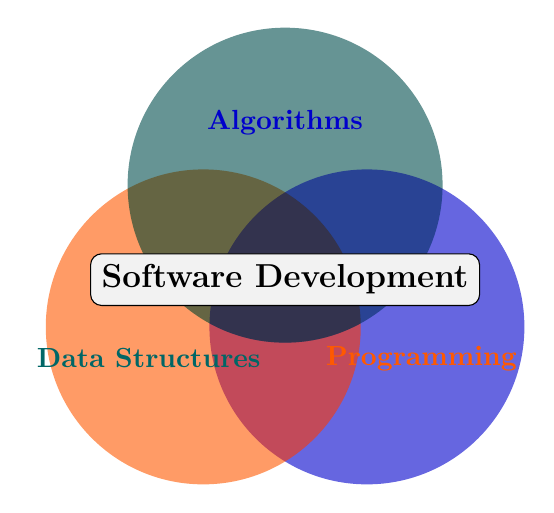
\begin{tikzpicture}
  % Draw three overlapping sets with new colors
  \begin{scope}[blend group=soft light]
    \fill[teal!60!black, opacity=0.6]   (90:1.2) circle (2);
    \fill[orange!70!red, opacity=0.6]   (210:1.2) circle (2);
    \fill[blue!80!black, opacity=0.6]   (330:1.2) circle (2);
  \end{scope}
  % Node labels with Computer Science synonyms
  \node[font=\bfseries, text=blue!80!black] at (90:2)    {Algorithms};
  \node[font=\bfseries, text=teal!80!black] at (210:2)   {Data Structures};
  \node[font=\bfseries, text=orange!70!red] at (330:2)   {Programming};
  \node[font=\large\bfseries, draw=black, fill=gray!10, rounded corners, inner sep=4pt] at (0,0) {Software Development};
\end{tikzpicture}
\end{document}